\chapter{Kybernetická bezpečnosť}
\phantomsection

S čoraz na väčšou informatizáciou naprieč všetkými odvetviami života, je nutnosťou riešiť aj zabezpečenie systémov, infraštruktúry a dát. Kybernetická bezpečnosť je bez pochýb jednou z najdiskutovanejších tém 21. storočia.
 
Podľa zistení z roku 2018 takmer polovica útokov smeruje na malé firmy, ktoré bezpečnosť riešia iba minimálne alebo vôbec. Predpokladá sa, že pre rok 2019 bude na kybernetickú bezpečnosť minutých 6 miliárd dolárov, naopak škody spôsobené kybernetickými útokmi presiahnu jednu miliardu dolárov a veľmi záškodné útoky typu \zkratka{zkDDoS} by mali vzrásť až šesťnásobne. \cite{Milkovich3122018} 

Vyššie zmienené predpovede len potvrdzujú dôležitosť kybernetickej  bezpečnosti pri návrhu, implementácie, nasadzovaní a prevádzke informačných technológií.




\section{Vybrané pojmy z kybernetickej bezpečnosti}
\begin{itemize}
	\item Informačné aktívum (Asset)\,--\,čokolvek, čo je nutné chránit, napr. dáta, fyzická informačná infraštruktúra, systémy \cite{McMillan2018}.\\
	
	\item Zraniteľnosť (Vulnerability)\,--\,neprítomnosť alebo nedostatočné opatrenia na zabezpečenie. Zraniteľnosť môže byť prítomná hardvéri, softvéri alebo samotnom užívateľovi \cite{McMillan2018}.\\
	
	\item Hrozba (Threat)\,--\,vzniká v prípade odhalenia alebo zneužitia zraniteľnosti. Zároveň platí, že hrozbou je aj zraniteľnosť, ktorá doposiaľ nebola neidentifikovaná \cite{McMillan2018}.\\
	
	\item Útočník (Threat agent)\,--\,entita, ktorá zneužije zraniteľnosť \cite{McMillan2018}.\\
    
    \item Riziko (Risk)\,--\,pravdepodobnosť, že útočník využije zraniteľnosť, pričom príde k dopadu na systém alebo infraštruktúru \cite{McMillan2018}.\\
  	
  	\item Útok na bezpečnosť (Security attack/Explotation)\,--\,krok, ktorý kompromituje bezpečnosť informačného aktíva \cite{Vyncke2008}.\\
  	    
	\item Bezpečnostný mechanizmus (Security mechanism)\,--\,proces, ktorý je navrhnutý na detegovanie, prevenciu a zotavenie z útoku na bezpečnosť. \\
	
	\item Protiopatrenie (Countermeasure)\,--\,ochranné opatrenie, ktoré znižuje riziko \cite{McMillan2018}.\\
	
	\item Expozícia informačného aktíva (Exposure)\,--\,dochádza k nej ak je aktívum vystavené stratám nedostatočným alebo neprítomným zabezpečením \cite{McMillan2018}.\\
	
\end{itemize}

	\begin{figure}[!h]
	\begin{center}
		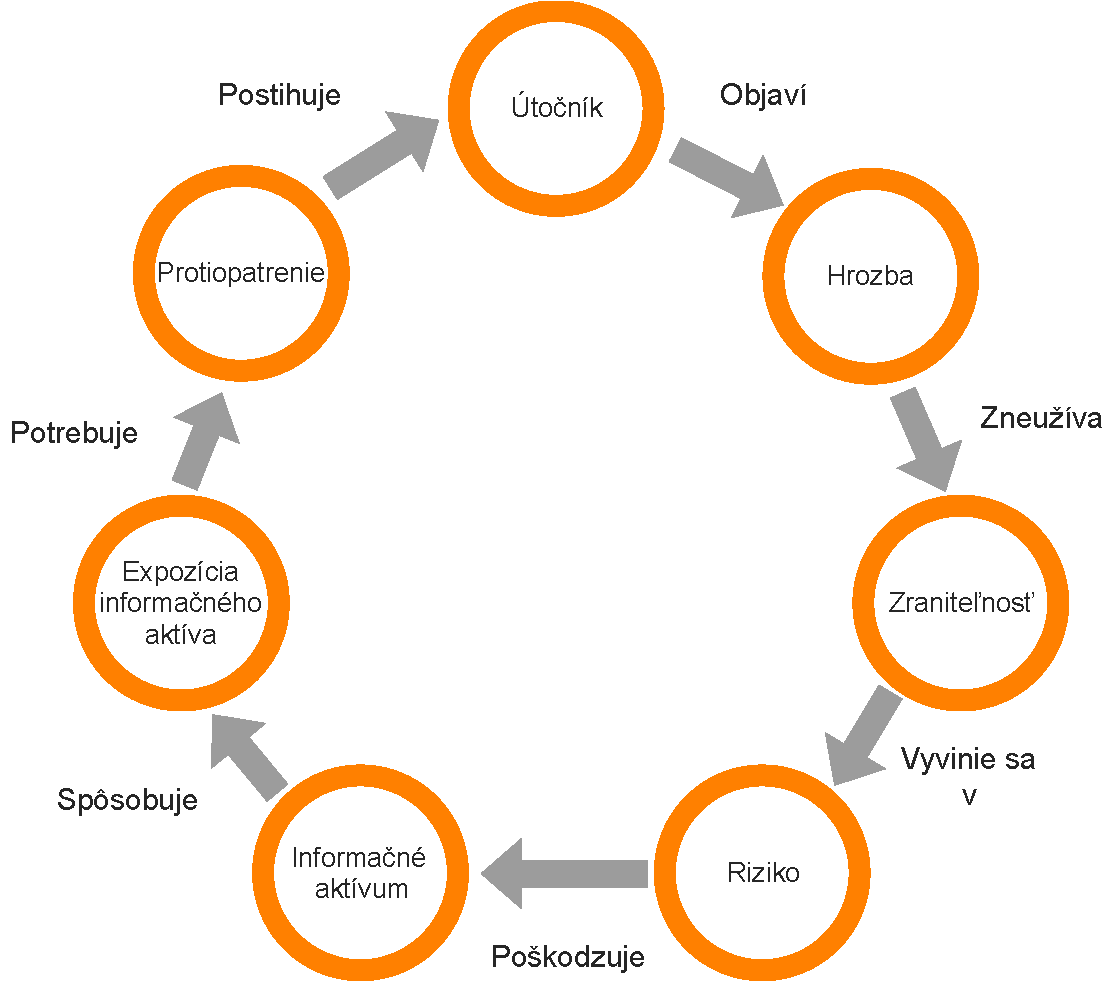
\includegraphics[scale=0.5]{obrazky/sec_cycle.pdf}
	\end{center}
	\caption[Koncept bezpečnosti a vzájomné vzťahy pojmov]{Koncept bezpečnosti a vzájomné vzťahy pojmov \cite{McMillan2018}}
	\label{sec-cycle}
	\end{figure}

Na obrázku \ref{sec-cycle} je možné vidieť vzájomnú interakciu medzi pojmami. Zároveň je nutné si uvedomiť, že takýto cyklus nie je v systéme alebo infraštruktúre jeden a taktiež môže vzniknúť niekoľko paralelných cyklov pričom každý môže mať počiatok v inom uzle. Je dobré myslieť na to, že jednotlivé cykly môžu na seba vplývať, napríklad jedno protiopatrenie môže postihnúť viacero útočníkov využívajúcich rôzne hrozby. 

\


\section{Ciele sieťovej bezpečnosti}
Bezpečnosť počítačovej siete, tak ako aj iných podoblastí kybernetickej bezpečnosti je založená na troch základných princípoch známych ako \zkratka{zkCIA}. Bezpečnosť musí pokryť všetky tri aspekty popísané týmto modelom, pričom narušenie čo i len jednej zložky má za následok nesplnenie celkového zabezpečenia \cite{Vyncke2008}. 

\subsection{Triáda CIA}

\begin{itemize}
	\item Confidentiality (Dôvernosť)\,--\,zabránenie prístupu k dátam alebo informáciám neoprávneným osobám. Na zaistenie tejto požiadavky sa najčastejšie používa šifrovanie, ale aj autentizácia a autorizácia. Jej strata vedie k neoprávnenému zverejnenie informácií. \cite{McMillan2018}
	
	\item Integrity (Integrita)\,--\,dáta alebo informácie sú zabezpečené proti neautorizovanej modifikácií a poškodeniu. Týmto zaisťujem konzistenciu dát pri prenose alebo uchovaní na médiu. Integritu zaisťujeme hašovacími funkciami prípadne za pomoci \zkratka{zkACL}. \cite{McMillan2018}
	
	\item Availability (Dostupnosť)\,--\,dáta alebo informácie sú dostupné iba pre určité entity v daný čas a miesto. \cite{McMillan2018}

	\begin{figure}[!h]
		\begin{center}
			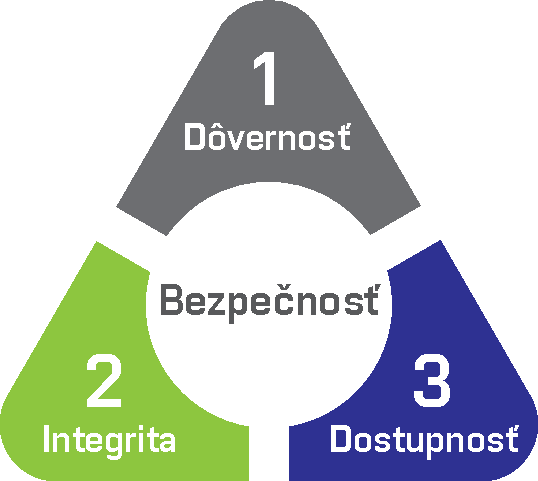
\includegraphics[scale=0.6]{obrazky/cia.pdf}
		\end{center}
		\caption[Triáda dôvernosť, integrita a dostupnosť]{Triáda dôvernosť, integrita a dostupnosť \cite{Vyncke2008}}%{CIA triáda\footnotemark}				
\label{cia}
\end{figure}
%\footnotetext{Zdroj: https://www.comtact.co.uk/blog/what-is-the-cia-triad}
\end{itemize}

	Aj keď triáda \zk{zkCIA} definuje ciele na zaistenie bezpečnosti, tak niektorí odborníci ju nepovažujú za dostatočnú a zavádzajú ďalšie dve podmienky a pojmy:\\
	\\
	\begin{itemize}
		\item Authencity (Autenticita)\,--\,overenie originálnosti a platnosti správy a identity jej pôvodcovi. Najčastejšie sa na zaistenie tejto podmienky využívajú certifikáty. \cite{Stallings2011}
		\item Accountability (Sledovateľnosť)\,--\,identifikácia prístupu k informáciám a vysledovateľnosť bezpečnostných incidentov v prípade využitia forenznej analýzy. Väčšinou je táto požiadavka zaistená záznamom činnosti v systéme formou logu. \cite{Stallings2011}
	\end{itemize}





\newpage
\section{Pasívne a aktívne útoky}
Útoky na bezpečnosť môžu byť rozdelené do dvoch skupín. Jednou skupinou je pasívny útok, kde nepozmeňuje útočník pôvodné dáta a nevplýva na príjemcu týchto dát. Druhou možnosťou je aktívny útok, pri ktorom sú buď pozmenené dáta doručené príjemcovi alebo je obeť nejakým spôsobom ovplyvňovaná, napríklad zasielaním falošných informácií. \cite{Vyncke2008}

\begin{figure}[H]
	\begin{center}
		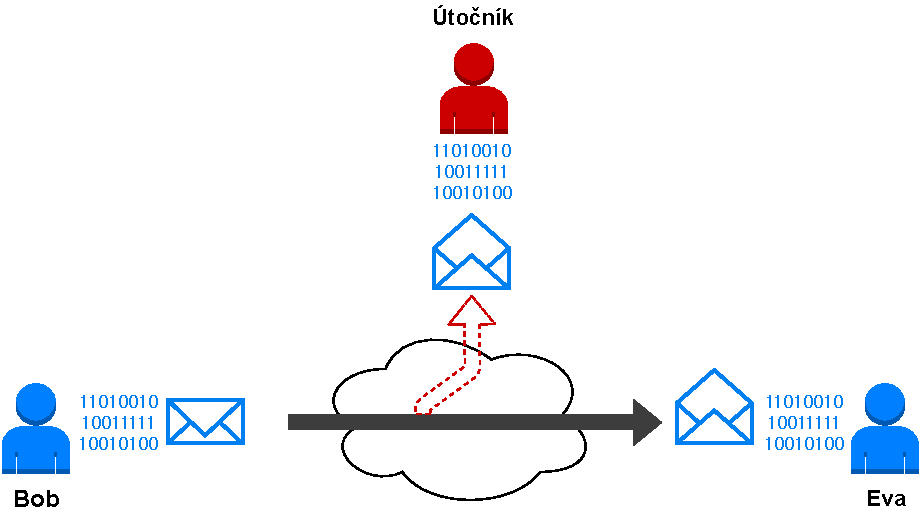
\includegraphics[scale=0.65]{obrazky/passive-attack.pdf}
	\end{center}
	\caption[Pasívny útok]{Pasívny útok \cite{Stallings2011}}
	\label{passive-attack}
\end{figure}

Pri pasívnom útoku, ktorý je znázornený na obrázku \ref{passive-attack} ide útočníkovi prevažne o zachytenie prenášanej komunikácie a monitorovanie a  analýzu prevádzky. Odposluch a zobrazenie obsahu dát je účinné hlavne pri nepoužití šifrovania správ medzi koncovými bodmi alebo aj pri použití slabých šifier, krátkych kľúčov a nedostatočne bezpečných hesiel. Monitorovanie prevádzky, respektíve analýza komunikácie je možná aj pri použití šifrovania, keďže každá komunikácia je charakteristická určitým vzorom. Pasívne útoky je nesmierne obtiažne detegovať nakoľko nemodifikujú dáta pri prenose. Najúčinnejšia obrana je použitie dostatočne silných šifier na zabezpečenie dát. Jeden z pasívnych útokov sa hojne využíva aj pri prevencii v \zkratka{zkIDS} a \zkratka{zkIPS}, kde bez analýzy prevádzky by nebolo možné zabezpečiť sieť. Pasívnymi útokmi sa nespôsobuje škoda na systéme alebo infraštruktúre, ale hrozba spočíva v narušení dôvernosti.

\begin{figure}[H]
	\begin{center}
		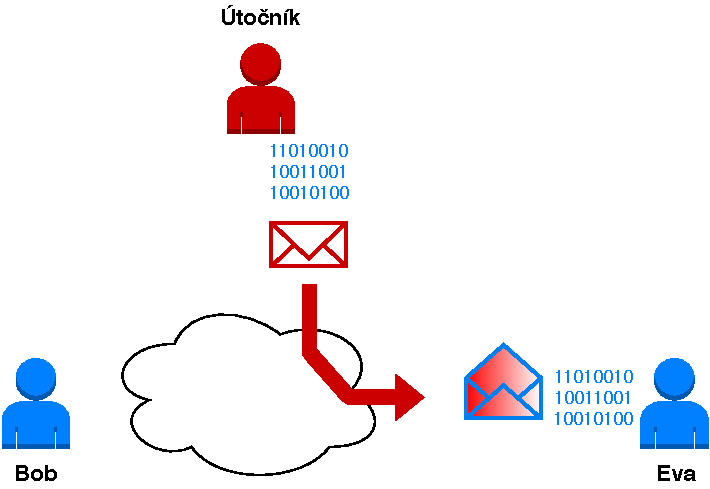
\includegraphics[scale=0.65]{obrazky/active-attack-masq.pdf}
	\end{center}
	\caption[Aktívny útok maškaráda]{Aktívny útok maškaráda \cite{Stallings2011}}
	\label{active-attack-masq}
\end{figure}

\begin{figure}[H]
	\begin{center}
		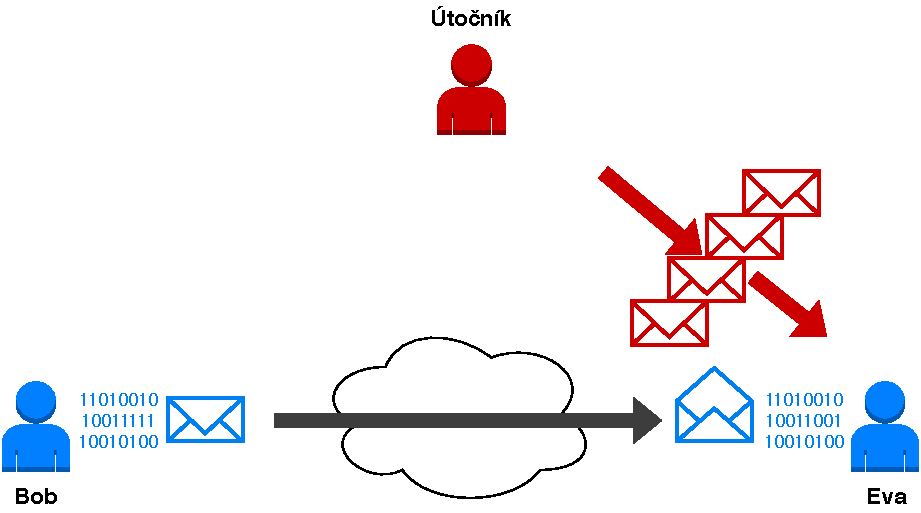
\includegraphics[scale=0.65]{obrazky/active-attack-dos.pdf}
	\end{center}
	\caption[Aktívny útok DOS]{Aktívny útok DOS \cite{Stallings2011}}
	\label{active-attack-dos}
\end{figure}

\begin{figure}[H]
	\begin{center}
		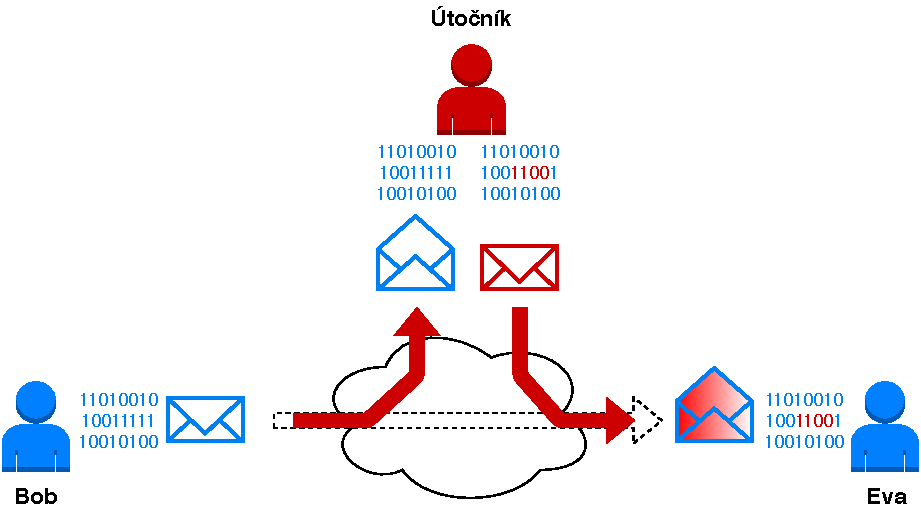
\includegraphics[scale=0.65]{obrazky/active-attack-mod.pdf}
	\end{center}
	\caption[Aktívny útok modifikácia správy]{Aktívny útok modifikácia správy \cite{Stallings2011}}
	\label{active-attack-mod}	
\end{figure}

\begin{figure}[H]
	\begin{center}
		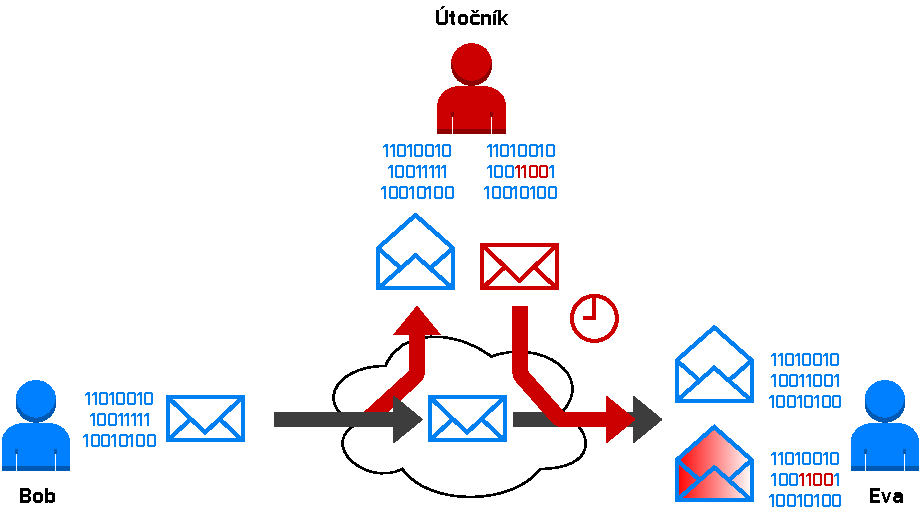
\includegraphics[scale=0.65]{obrazky/active-attack-reply.pdf}
	\end{center}
	\caption[Aktívny útok prehratím]{Aktívny útok prehratím \cite{Stallings2011}}
	\label{active-attack-reply}
\end{figure}

Aktívne útoky sú sofistikovanejšie ako pasívne, modifikujú dáta alebo vytvárajú falošné, o ktorých prijímateľ predpokladá, že prišli od zdroja, s ktorým pôvodne komunikoval. Hrozby, ktoré môžu týmito útokmi nastať sú strata integrity, teda modifikácia dát a ohrozenie dostupnosti pričom vždy dochádza ku škode na systéme alebo infraštruktúre. Maškaráda je prvým z aktívnych útokov, kde ako je možné vidieť na obrázku \ref{active-attack-masq}, útočník vytvára falošnú správu, ktorú zasiela obeti a tá sa domnieva, že komunikuje s pôvodným zdrojom, v našom prípade Bobom. Príkladom aktívneho útoku je aj útok odoprenia služby \ref{active-attack-dos}, kde sa vytvárajú falošné dáta generované vysokou frekvenciou za účelom odstaviť systém alebo infraštruktúru, ktorá nezvláda spracovanie toľkých požiadaviek, keďže nebola na takúto záťaž dimenzovaná. Tretím aktívnym útokom \ref{active-attack-mod} je modifikácia správy útočníkom pri prechode komunikačným kanálom, ktorý sa realizuje rôznymi technikami podvrhnutia zdroja alebo identity. Posledným útokom je útok prehratím \ref{active-attack-reply}, čo je útok veľmi podobný predchádzajúcemu, akurát obeť obdrží najprv pôvodnú nepozmenenú správu a následne po určitom čase aj modifikovanú správu od útočníka.  




